% Created 2024-07-03 Wed 18:55
% Intended LaTeX compiler: pdflatex
\documentclass[10pt,table,dvipsnames,compress]{beamer}
\usepackage[utf8]{inputenc}
\usepackage[T1]{fontenc}
\usepackage{graphicx}
\usepackage{longtable}
\usepackage{wrapfig}
\usepackage{rotating}
\usepackage[normalem]{ulem}
\usepackage{amsmath}
\usepackage{amssymb}
\usepackage{capt-of}
\usepackage{hyperref}
\usetheme{default}
\useinnertheme{rounded}
\useoutertheme[subsection=false]{miniframes}
\date{}
\title{Riskmaps for carbon credit certification}
\title[riskmaps]{Riskmaps for carbon credit certification}
\definecolor{darkgreen}{RGB}{34,139,34} % vert moyen
\usepackage{lmodern}
\usepackage{pgf}
\usepackage{color}
\usepackage[english,french]{babel}
\definecolor{vertmoyen}{RGB}{51,110,23} % vert moyen
\definecolor{blueFRB}{HTML}{31859c}
\usecolortheme[named=blueFRB]{structure}
\usepackage{tabularx} % varier la largeur du tableau
\usepackage{layout}
\setlength{\LTleft}{-5cm plus 1 fill}
\setlength{\LTright}{-5cm plus 1 fill}
\usepackage{booktabs}
\usepackage{arydshln} %% dashlines for tabular
\newcommand{\logit}{\text{logit}}
\newcommand{\bs}[1]{\boldsymbol{#1}}
\newcommand{\R}{\textnormal{\sffamily\bfseries R}}
\newcommand{\pkg}[1]{{\fontseries{b}\selectfont #1}}
\newcolumntype{C}[1]{>{\centering\arraybackslash}m{#1}}

\setbeamertemplate{footline}[frame number]
\setbeamertemplate{frametitle}{%
\usebeamerfont{frametitle}\insertframetitle%
\vphantom{g} % To avoid fluctuations per frame
\par
\centering 
\includegraphics[width=\textwidth]{figs/Barre_couleur}
}
\beamertemplatenavigationsymbolsempty

% Logo
\newif\ifplacelogo % create a new conditional
\logo{\ifplacelogo
\includegraphics[width=0.5\textwidth]{figs/partners_logos}\fi}

%Call table of contents at the beginning of each section
\AtBeginSection[]{
\placelogotrue
\begin{frame}
\frametitle{Plan}
\begin{columns}[c]
\begin{column}{0.5\textwidth}
\tableofcontents[sections=1,currentsection]
\vspace{0.5cm}
\tableofcontents[sections=2,currentsection]
\end{column}
\begin{column}{0.5\textwidth}
\tableofcontents[sections=3,currentsection]
\vspace{0.5cm}
\tableofcontents[sections=4,currentsection]
\end{column}
\end{columns}
\end{frame}
\placelogofalse
}

\AtBeginSubsection[]{}

\hypersetup{
colorlinks=true,
linkcolor=Black,
filecolor=Maroon,
citecolor=Blue,
urlcolor=Maroon}

% Disable monospaced font for URLs
\urlstyle{same}

\hypersetup{
 pdfauthor={Ghislain Vieilledent},
 pdftitle={Riskmaps for carbon credit certification},
 pdfkeywords={},
 pdfsubject={},
 pdfcreator={Emacs 29.3 (Org mode 9.6.15)}, 
 pdflang={English}}
\begin{document}


% {
%   % Use background image
%   \usebackgroundtemplate{%
%     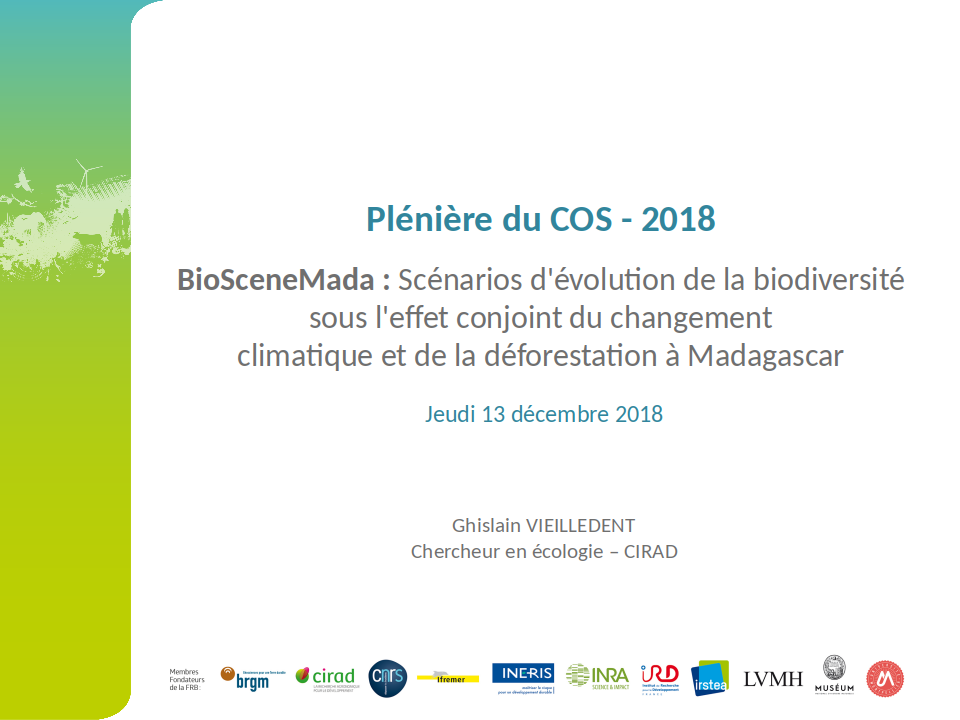
\includegraphics[height=\paperheight,width=\paperwidth]{figs/Masque.png}
%   }
%   \setbeamertemplate{navigation symbols}{}
%   % Remove shadow from block
%   \setbeamertemplate{blocks}[rounded][shadow=false]
%   \begin{frame}[plain]
%   \end{frame}
% }

% Title page
{
  \setbeamertemplate{navigation symbols}{}
  \begin{frame}[plain, noframenumbering]
  \begin{center}
  \small{\textbf{FAO workshop -- Santa Marta (Colombia), July 2024}}
  \end{center}
  \vspace{-0.5cm}
  \titlepage % Presentation first page
  \vspace{-3cm}
  \begin{center}
    
\includegraphics[width=\textwidth]{figs/Barre_couleur}
    
    \vspace{0.25cm}
    
    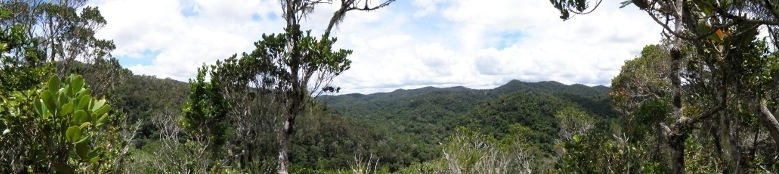
\includegraphics[width=10cm]{figs/Banniere}
    
    \small{Ghislain VIEILLEDENT$^{1}$\hspace{0.25cm}Thomas ARSOUZE$^{1}$\hspace{0.25cm}FAO team$^{2}$}
      
    \vspace{0.25cm}
    
    {\scriptsize
      \begin{tabular}{l}
        $[1]$ \textbf{Cirad} UMR AMAP, $[2]$ \textbf{FAO} Rome and Latin America
      \end{tabular}
    }
    
    
\includegraphics[width=0.8\textwidth]{figs/partners_logos}
    
  \end{center}
  \end{frame}
}

% %%%%%%%%%%%%%%%%%%%%%%%%%%%%%%%%%%%%%%%%%%%%%%%%%%%%%%%%%%%%%%%%

\placelogotrue
\begin{frame}
  \frametitle{Plan}
  \begin{columns}[c]
    \begin{column}{0.5\textwidth}
      \tableofcontents[sections=1]
      \vspace{0.5cm}
      \tableofcontents[sections=2]
    \end{column}
    \begin{column}{0.5\textwidth}
        \tableofcontents[sections=3]
        \vspace{0.5cm}
        \tableofcontents[sections=4]
    \end{column}
  \end{columns}
\end{frame}
\placelogofalse

\section{Introduction}
\label{sec:orga12b708}

\subsection{Improving certification methodologies}
\label{sec:org13825aa}

\begin{frame}[label={sec:org6acac64}]{Several criticisms}
Several criticisms were addressed to previous REDD+ methodologies for carbon credit certification accusing them to oversell credits.

\begin{itemize}
\item \textbf{Non-additionnality}: Emissions reductions would have happened anyway. Inflated project-level baselines. Jurisdictional reference levels are reasonably good predictors of future trends.
\item \textbf{Leakage}: The larger the area covered by a REDD+ initiative, the lower the leakage risk.
\item \textbf{Reversal}: Jurisdictions are less likely than projects to have their forest carbon stocks decimated by a disturbance event.
\end{itemize}

Frances Seymour (WRI): \href{https://www.wri.org/insights/insider-4-reasons-why-jurisdictional-approach-redd-crediting-superior-project-based}{4 Reasons Why a Jurisdictional Approach for REDD+ Crediting Is Superior to a Project-Based Approach}.
\end{frame}

\begin{frame}[label={sec:orgf7bee1f}]{New jurisdictional approach}
\begin{block}{Deforestation intensity}
\begin{itemize}
\item Baseline activity data or Forest Reference Emission Level at the jurisdictional level
\item Amount of deforestation.
\item Deforestation ``quantity'' or ``intensity''.
\end{itemize}
\end{block}

\begin{block}{Spatial deforestation risk}
\begin{itemize}
\item Map of the deforestation risk at the jurisdictional level.
\item Spatial relative probability of deforestation.
\item Deforestation ``location''.
\end{itemize}
\end{block}
\end{frame}

\subsection{Allocating deforestation to projects}
\label{sec:orga125820}

\begin{frame}[label={sec:org82dcc11}]{Risk map at the jurisdictional level}
\begin{columns}
\begin{column}{0.5\columnwidth}
\begin{block}{Objectives}
\begin{itemize}
\item Identifying hot-spots/cold-spots of deforestation.
\item Classifying forest pixels by risk of being deforested.
\item One unique model for the whole jurisdiction (no methodological discrepancies between projects).
\item Use this map to allocate deforestation (estimated for the jurisdiction) per project.
\end{itemize}
\end{block}
\end{column}

\begin{column}{0.5\columnwidth}
\begin{figure}[htbp]
\centering
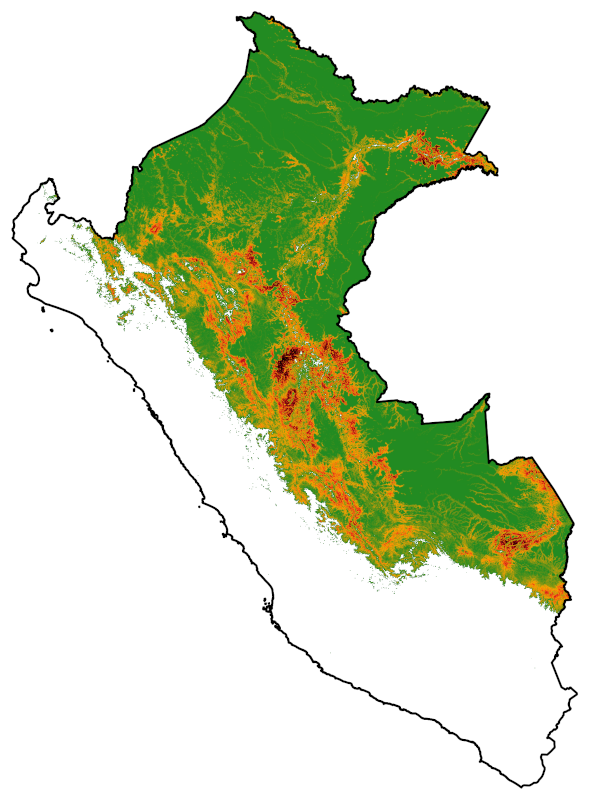
\includegraphics[width=4cm]{figs/prob_PER.png}
\caption{Map of the deforestation risk for Perou.\newline \textcolor{darkgreen}{Green}: low, \textcolor{red}{Red}/\textbf{Black}: high.}
\end{figure}
\end{column}
\end{columns}
\end{frame}

\begin{frame}[label={sec:orge2adc64}]{Allocating deforestation to projects}
\begin{itemize}
\item Jurisdictional risk map: a map with class of deforestation risk.
\item Obtaining a deforestation density map:\newline Class of defor. risk [1, 2, \ldots{}, \(I\)] \(\rightarrow\) Defor. density (ha/yr/pixel).
\item Can be used to allocate deforestation per project.
\end{itemize}

\begin{figure}[htbp]
\centering
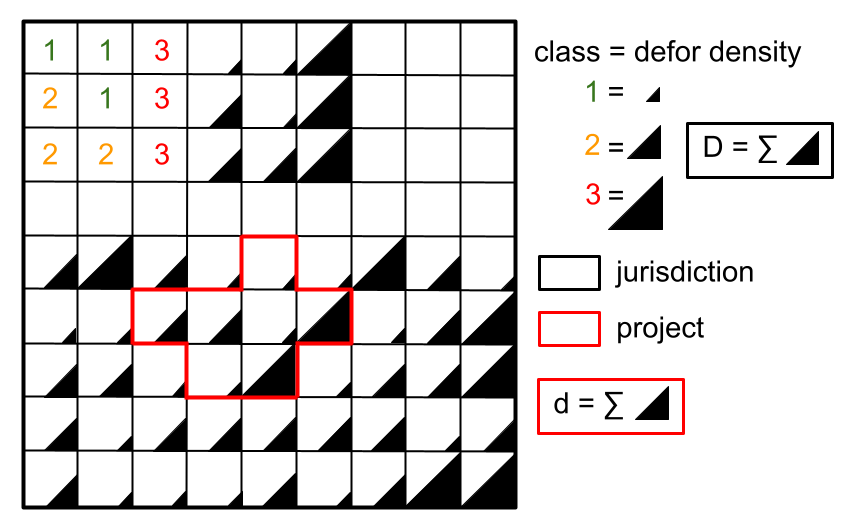
\includegraphics[width=8cm]{figs/get_started/allocation.png}
\caption{Allocating deforestation to projects within the jurisdiction.}
\end{figure}
\end{frame}

\section{Verra's tool VT0007 for risk maps}
\label{sec:orgfec914b}

\subsection{VT0007 methodology}
\label{sec:orgaa7c778}

\begin{frame}[label={sec:org62bb88c}]{VT0007 methodology}
\begin{itemize}
\item Developed by Clark University (J. R. Eastman and R. G. Pontius Jr.) for Verra.
\item \textbf{Aim}: Obtaining the best risk map possible at the jurisdictional level.
\end{itemize}

\begin{block}{Basic steps}
\begin{enumerate}
\item Use a reasonably good reference model to map the deforestation risk.
\item Let the user propose alternative maps from alternative models.
\item Validation step: check that alternative models are better than the benchmark model.
\item Use the best alternative map to allocate deforestation.
\end{enumerate}
\end{block}
\end{frame}

\begin{frame}[label={sec:org7ca12e9}]{Modelling periods}
\begin{center}
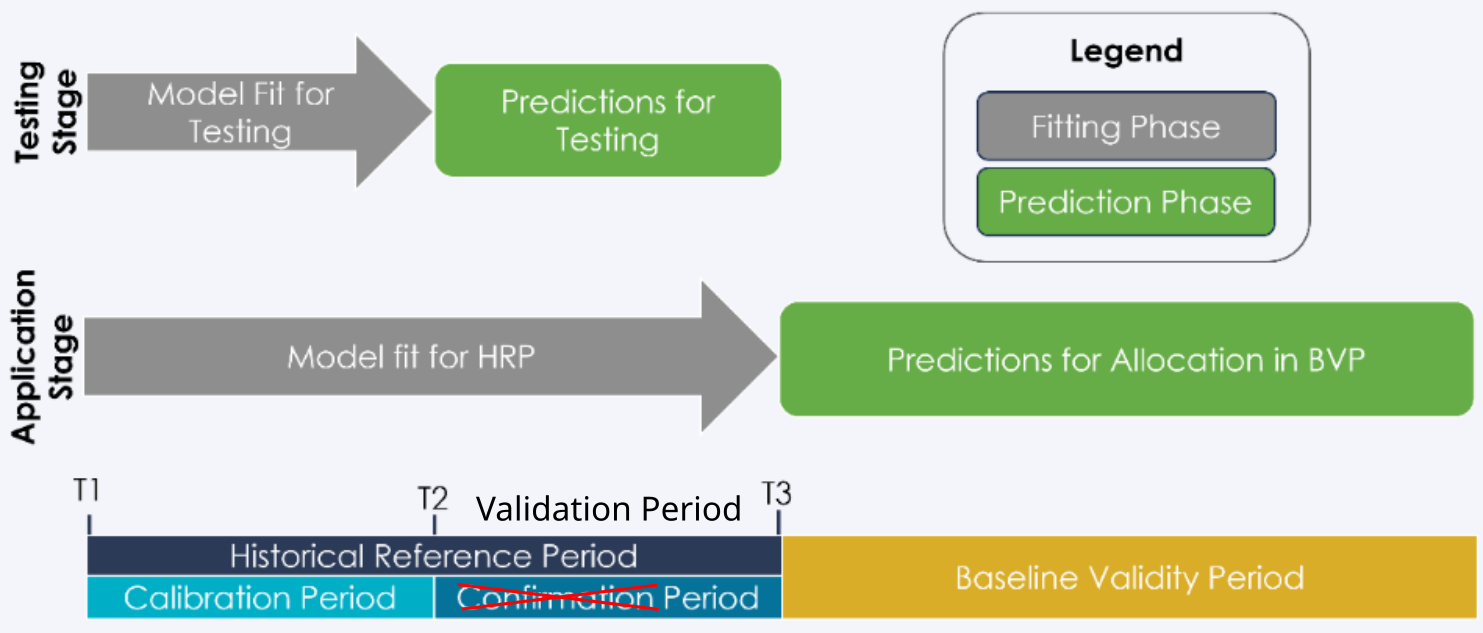
\includegraphics[width=9cm]{figs/get_started/periods.png}
\end{center}

\begin{itemize}
\item Three dates: t1, t2, t3.
\item Four periods: calibration, validation, historical, (baseline validity period).
\item Why different periods: model predictions must be compared with \textbf{independent data} (validation period).
\item To forecast after t3, we want to use as much data as possible (historical period).
\end{itemize}
\end{frame}

\subsection{Benchmark model}
\label{sec:org788a721}

\begin{frame}[label={sec:org9ee015b}]{Benchmark model}
\end{frame}

\begin{frame}[label={sec:orgac64b3b}]{Deforestation density}
\end{frame}

\subsection{Alternative models and validation}
\label{sec:org503398b}

\begin{frame}[label={sec:org800b7aa}]{Alternative models}
\end{frame}

\begin{frame}[label={sec:orgecbe8f8}]{Validation}
\end{frame}

\subsection{Validation ad time periods}
\label{sec:orgc872f77}

\begin{frame}[label={sec:org295ce25}]{Calibration, validation, and historical periods}
\end{frame}

\begin{frame}[label={sec:org053acbb}]{Validation procedure}
\end{frame}

\subsection{Verra/UClark software for V0007}
\label{sec:org94f26f5}

\begin{frame}[label={sec:org588bdc8}]{Verra/UClark software}
\url{https://github.com/ClarkCGA/UDef-ARP/tree/v2.09}

\begin{itemize}
\item User must provide fcc, distance to forest edge raster, subjurisdictional borders.
\item Benchmark model.
\item Validation.
\end{itemize}
\end{frame}

\begin{frame}[label={sec:org6715739}]{Limitations}
\begin{itemize}
\item Not tool to help prepare the data.
\item No tool to develop the alternative model.
\item Windows only.
\item Require a computer with high RAM for large jurisdiction: all raster inputs are stored in RAM during processing. Therefore, large jurisdictions will require substantial RAM allocations (e.g., 64Gb).
\item Several remarks:
\end{itemize}
\end{frame}

\section{Software for modelling deforestation}
\label{sec:orga03d40b}

\subsection{Existing software}
\label{sec:orgf2891b2}

\begin{frame}[label={sec:orgd98f5de}]{Existing software}
\begin{itemize}
\item Dinamica EGO, CLUE, TerraSet (Clark U.).
\end{itemize}
\end{frame}

\subsection{Limitations}
\label{sec:orga4b34a6}

\begin{frame}[label={sec:org3c47cc4}]{Limitations}
\begin{itemize}
\item All are not open source (transparency).
\item Difficulty to reproduce the results (transparency, reproducibility).
\item Large rasters on large jurisdiction ?
\item No scripting: not well adapted to repeat computation.
\end{itemize}
\end{frame}

\section{Conclusion}
\label{sec:org5e543c5}

\subsection{A not so simple methodology}
\label{sec:org04024c2}

\begin{frame}[label={sec:orgdd2ff0a}]{A not so simple methodology}
\end{frame}

\subsection{Need for an integrative tool: deforisk QGIS plugin}
\label{sec:orgd3a7c15}

\begin{frame}[label={sec:org0508e15}]{Need for an integrative tool: the deforisk QGIS plugin}
\end{frame}

% %%%%%%%%%%%%%%%%%%%%%%%%%%%%%%%%%%%%%%%%%%%%%%%%%%%%%%%%%%

{
  % Use background image
  \usebackgroundtemplate{%
    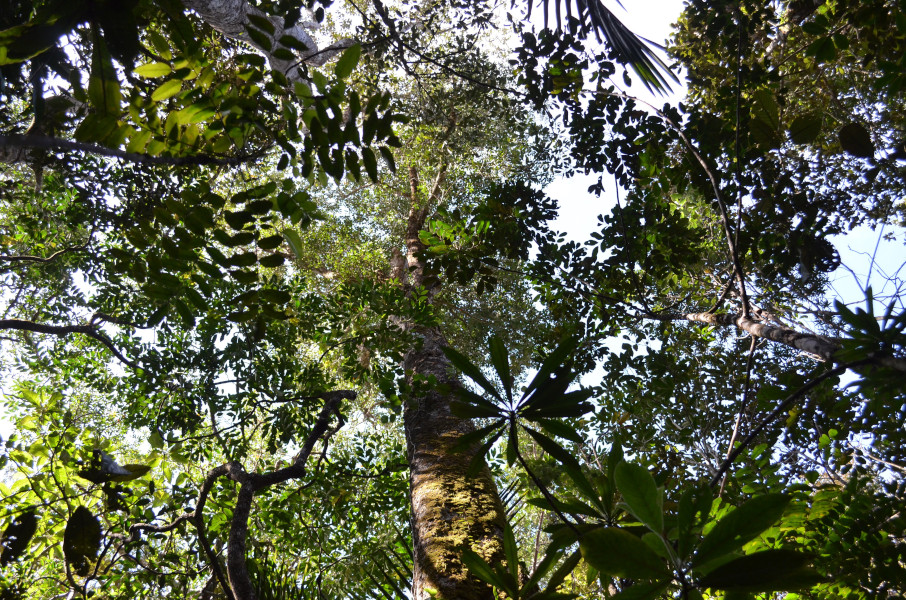
\includegraphics[keepaspectratio=true, height=\paperheight]{figs/Canopy-NC}
  }
  \setbeamertemplate{navigation symbols}{}
  % Remove shadow from block
  \setbeamertemplate{blocks}[rounded][shadow=false]
  \begin{frame}[plain]
  	\vspace*{\stretch{100}} 
    \begin{block}{}
      \begin{center}
        \ldots~Thank you for attention~\ldots \\
        \url{https://forestatrisk.cirad.fr} \\
        
\includegraphics[width=0.8\textwidth]{figs/partners_logos}
      \end{center}
    \end{block}
  \end{frame}
}
\end{document}
